% Code listing configuration for MATLAB
\lstset{
    language=Matlab,
    basicstyle=\ttfamily\small,
    keywordstyle=\color{blue},
    stringstyle=\color{purple},
    commentstyle=\color{green!60!black},
    numbers=left,
    numberstyle=\tiny\color{gray},
    breaklines=true,
    frame=single,
    captionpos=b
}

\section{Exercise 7.10: DFT basics}
\subsection{MATLAB Implementation}

Below is the MATLAB script dft\_delta.m. This script performs a Discrete Fourier Transform (DFT) calculation on a simple array labeled f consisting of zeros with a length of 10 and the first value set to one. The script then computes the Inverse Discrete Fourier Transform (IDFT) on the the subsequent array labeled F and achieves the original array f. 

\lstinputlisting[caption={MATLAB script \texttt{dft\_delta.m}}, label={lst:dft_delta}]{Code/dft_delta.m}


\subsection{Results}
\begin{figure}[H]
    \centering
    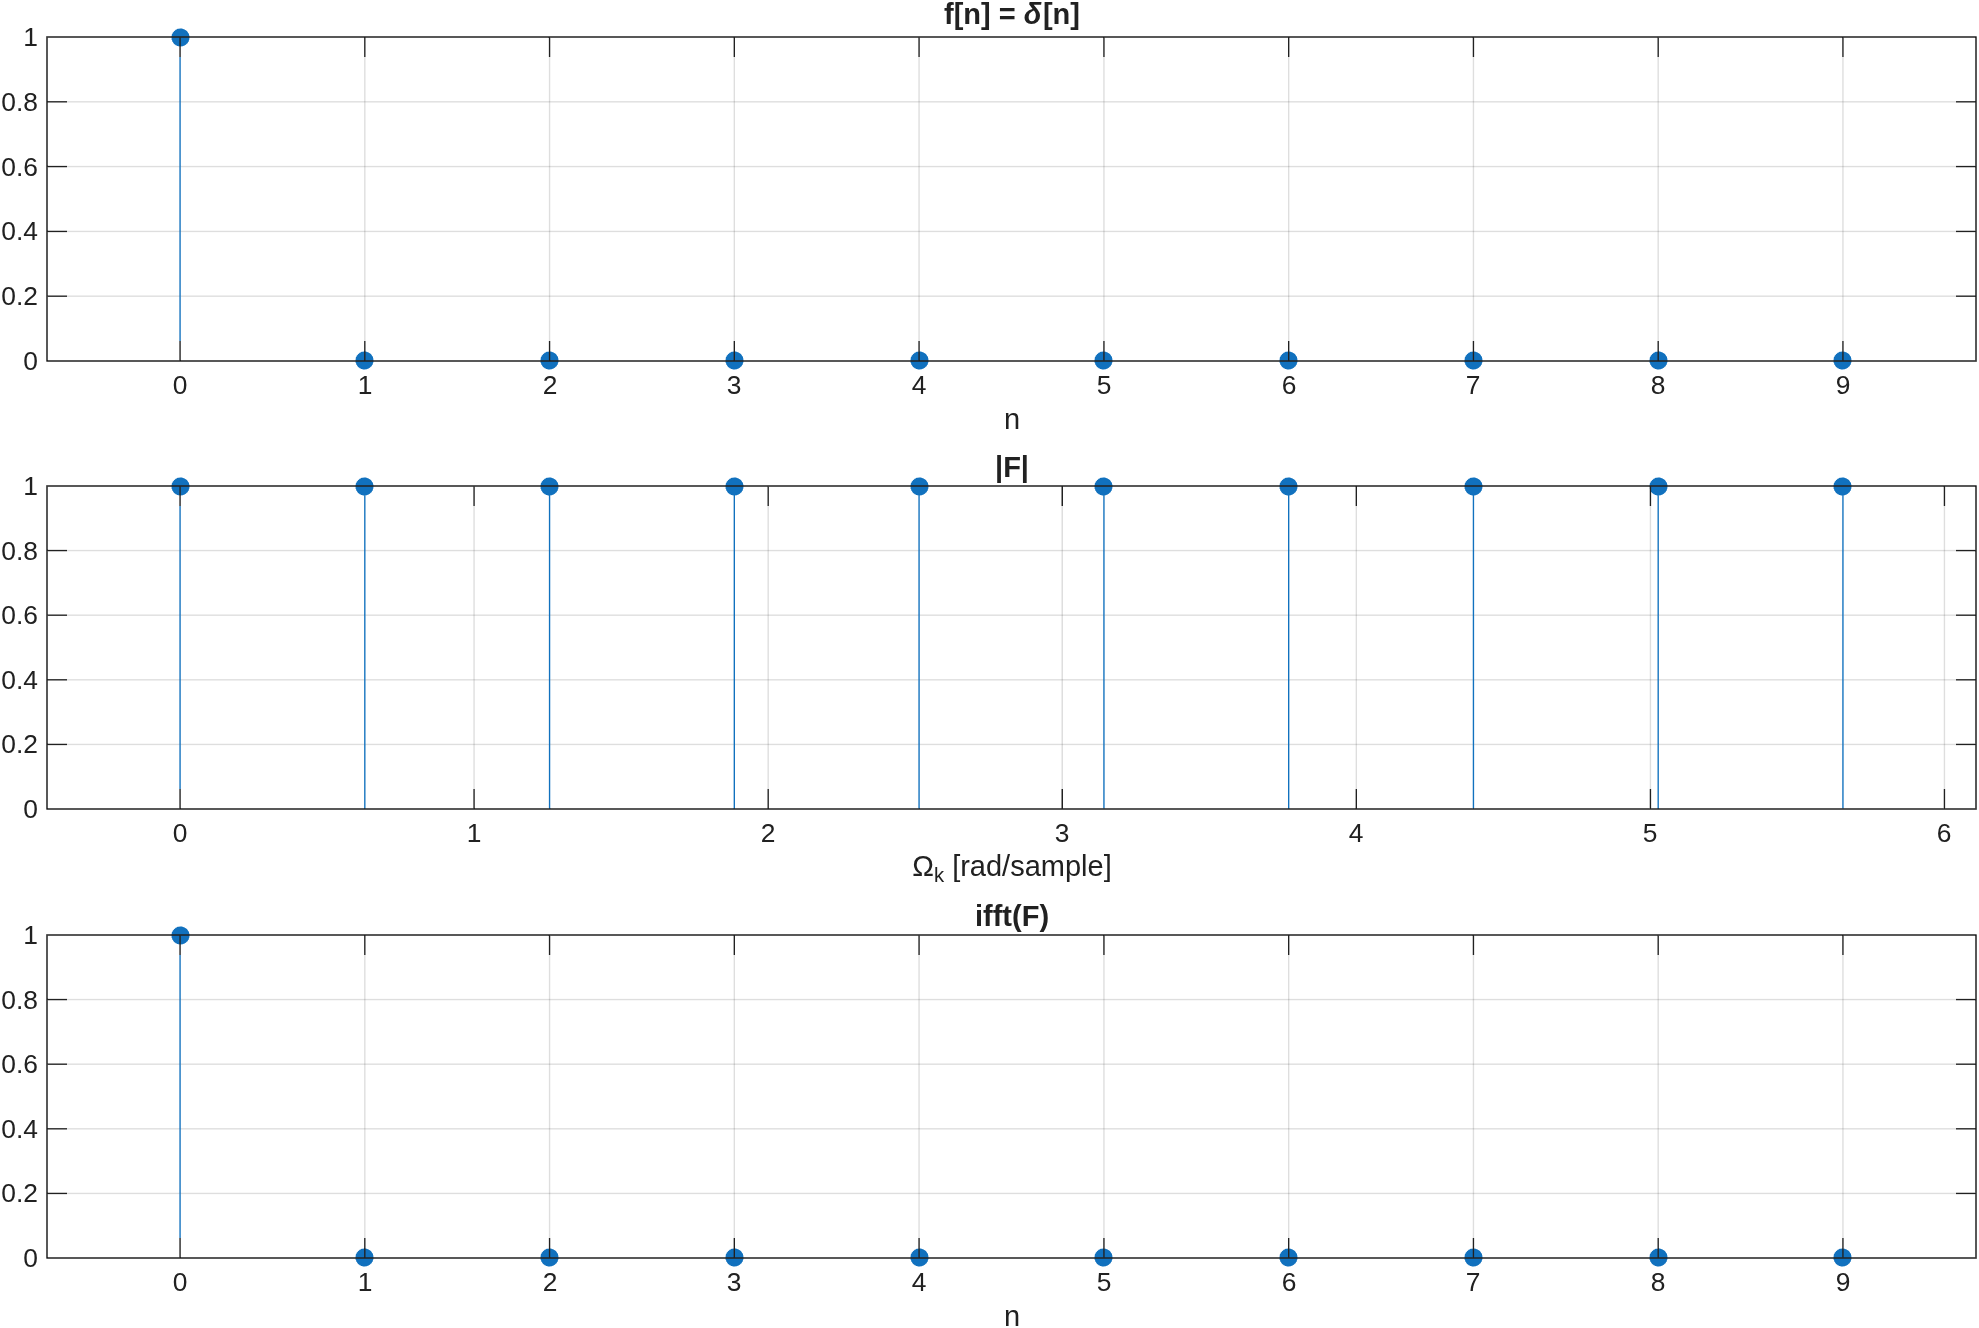
\includegraphics[width=0.8\linewidth]{Figures//7.10 Figures/Exercise 7 10 DFT Basics.png}
    \caption{Graphs}
    \label{fig:placeholder}
\end{figure}

\subsection{Results Analysis}
The DFT of a delta-peak function is F[k] = 1, here we see that same result when performing a DFT on f.